%\documentclass[tikz,border=10pt]{standalone}
\documentclass[]{standalone}
	%% Compile svg by running:
	%% latex example.tex #OR:  lualatex --output-format=dvi example.tex
	%% dvisvgm --bbox=10 example.dvi
	\usepackage{tikz}
	\usetikzlibrary{calc}
	
	\definecolor{col0}{RGB}{255, 51, 51}
	\definecolor{col1}{RGB}{215,255, 51}
	\definecolor{col2}{RGB}{ 51,255,133}
	\definecolor{col3}{RGB}{ 51,133,255}
	\definecolor{col4}{RGB}{215, 51,255}
	
	\begin{document}%
	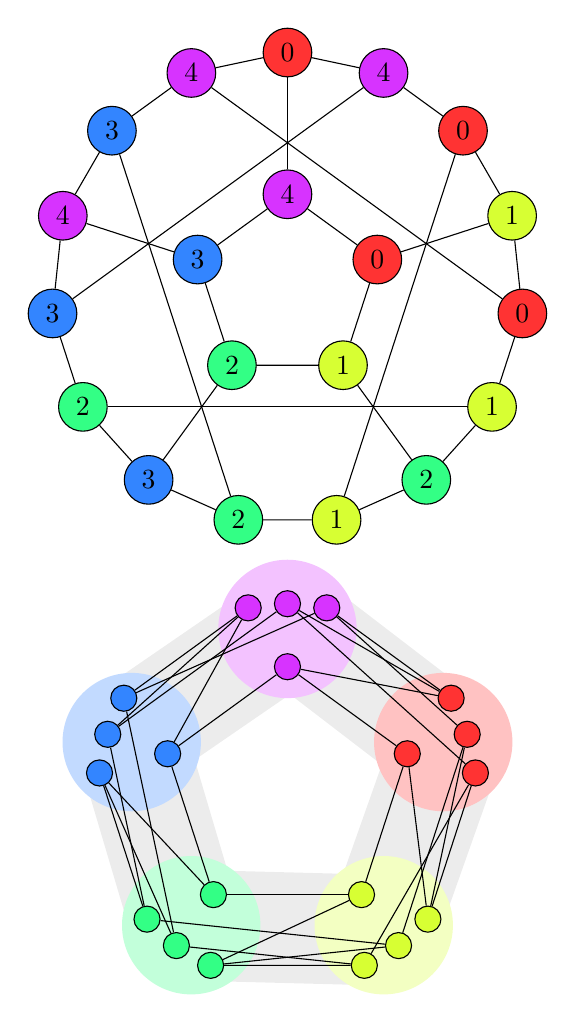
\begin{tikzpicture}[
		scale=0.8,rotate=90,every node/.style={draw,circle},
		C0/.style={fill=col0},
		C1/.style={fill=col1},
		C2/.style={fill=col2},
		C3/.style={fill=col3},			
		C4/.style={fill=col4}
	]
	
	%the flower snark graph J_5
	%vertices
		\foreach \x/\c in {0/4, 1/3,  2/2, 3/1, 4/0}
			\node[C\c] (u\x) at (\x * 72 :1.5) {\c};
		\foreach \x/\c in {0/0, 1/4,  2/3, 3/4, 4/3, 5/2, 6/3, 7/2, 8/1, 9/2, 10/1, 11/0, 12/1, 13/0, 14/4}
			\node[C\c] (v\x) at (\x * 24 :3.75) {\c};
	%edges
		\foreach \x in {0,...,4}
		{
			\pgfmathtruncatemacro{\xp}{mod(\x+1,5)};
			\draw (u\x) -- (u\xp);
			\pgfmathtruncatemacro{\xx}{3*\x};
			\draw (u\x) -- (v\xx);
			\pgfmathtruncatemacro{\xa}{3*\x+1};
			\pgfmathtruncatemacro{\xb}{mod(3*\x+11,15)};		
			\draw (v\xa) -- (v\xb);
		}
		\foreach \x in {0,...,14}	
		{
			\pgfmathtruncatemacro{\xp}{mod(\x+1,15)};
			\draw (v\x) -- (v\xp);
		}
	
	%the image of J_5 in C_5
	\begin{scope}[shift={(-8,0)}]
	%blob edges
		\foreach \x in {0,...,4}
		{
			\pgfmathtruncatemacro{\xp}{mod(\x+1,5)};
			\draw[gray!15!white,line width=40pt](\x * 72 :2.6) -- (\xp * 72 :2.7);
		}
	%blobs
		\foreach \x/\c in {0/4, 1/3,  2/2, 3/1, 4/0}
			\node[draw=none,fill=col\c!30!white,minimum size=50pt] (u\x) at (\x * 72 :2.6) {};
	%vertices
		\foreach \x/\c in {0/4, 1/3,  2/2, 3/1, 4/0}
			\node[C\c] (u\x) at (\x * 72 :2) {};
		\foreach \x/\c/\d in {0/0/2, 1/4/0,  2/3/0, 3/4/2, 4/3/1, 5/2/0, 6/3/2, 7/2/1, 8/1/0, 9/2/2, 10/1/1, 11/0/1, 12/1/2, 13/0/0, 14/4/1}
			\node[C\c] (v\x) at ((-72 - \c * 72 + \d*12-12 :3) {};
	%the same edges
		\foreach \x in {0,...,4}
		{
			\pgfmathtruncatemacro{\xp}{mod(\x+1,5)};
			\draw (u\x) -- (u\xp);
			\pgfmathtruncatemacro{\xx}{3*\x};
			\draw (u\x) -- (v\xx);
			\pgfmathtruncatemacro{\xa}{3*\x+1};
			\pgfmathtruncatemacro{\xb}{mod(3*\x+11,15)};		
			\draw (v\xa) -- (v\xb);
		}
		\foreach \x in {0,...,14}	
		{
			\pgfmathtruncatemacro{\xp}{mod(\x+1,15)};
			\draw (v\x) -- (v\xp);
		}		
	\end{scope}		
	\end{tikzpicture}%
	\end{document}